\documentclass[12pt,compress,english,utf8,t]{beamer}
\usepackage[ngerman]{babel}
\usepackage{calc}
\usepackage{ragged2e,wasysym,multicol,mathtools,mathdots}
\usepackage[protrusion=true,expansion=true]{microtype}
\usepackage{tikz,ifthen}
\usetikzlibrary{calc,shapes,shapes.callouts,shapes.arrows,patterns,fit,backgrounds,decorations.pathmorphing}
\usepackage{booktabs}
\hypersetup{colorlinks=true}

\graphicspath{{images/}}

\title{Large numbers, very large numbers and very very large numbers}
\author{Ingo Blechschmidt}
\date{December 17th, 2019}

%\usetheme{Warsaw}
\useinnertheme[shadow=true]{rounded}
\useoutertheme{split}
\usecolortheme{orchid}
\usecolortheme{whale}
\setbeamerfont{block title}{size={}}

\useinnertheme{rectangles}

\usecolortheme{seahorse}
\definecolor{mypurple}{RGB}{150,0,255}
\setbeamercolor{structure}{fg=mypurple}
\definecolor{myred}{RGB}{150,0,0}
\setbeamercolor*{title}{bg=myred,fg=white}
\setbeamercolor*{titlelike}{bg=myred,fg=white}

\usefonttheme{serif}
\usepackage[T1]{fontenc}
\usepackage{libertine}

\renewcommand{\_}{\mathpunct{.}\,}
\newcommand{\BB}{\mathbb{B}}
\newcommand{\M}{\mathcal{M}}
\newcommand{\R}{\mathrm{R}}
\newcommand{\NN}{\mathbb{N}}
\newcommand{\RR}{\mathbb{R}}

\setbeamertemplate{navigation symbols}{}

\setbeamertemplate{title page}[default][colsep=-1bp,rounded=false,shadow=false]
\setbeamertemplate{frametitle}[default][colsep=-2bp,rounded=false,shadow=false,center]

\newcommand{\hil}[1]{{\usebeamercolor[fg]{item}{\textbf{#1}}}}
\setbeamertemplate{frametitle}{%
  \vskip1em%
  \leavevmode%
  \begin{beamercolorbox}[dp=1ex,center]{}%
      \usebeamercolor[fg]{item}{\textbf{\textsf{\Large \insertframetitle}}}
  \end{beamercolorbox}%
}

\setbeamertemplate{footline}{%
  \leavevmode%
  \hfill%
  \begin{beamercolorbox}[ht=2.25ex,dp=1ex,right]{}%
    \usebeamerfont{date in head/foot}
    \insertframenumber\,/\,\inserttotalframenumber\hspace*{1ex}
  \end{beamercolorbox}%
  \vskip0pt%
}

\newcommand{\backupstart}{
  \newcounter{framenumberpreappendix}
  \setcounter{framenumberpreappendix}{\value{framenumber}}
}
\newcommand{\backupend}{
  \addtocounter{framenumberpreappendix}{-\value{framenumber}}
  \addtocounter{framenumber}{\value{framenumberpreappendix}}
}

\setbeameroption{show notes}
\setbeamertemplate{note page}[plain]

% Taken from Todd Lehman (CC-BY-SA) at https://tex.stackexchange.com/a/44920/32372

\newcommand{\setisprime}[1]{
  % Sets \isprime based on #1.
  \ifnum#1=1 \gdef\isprime{0} \else \gdef\isprime{1} \fi
  \foreach \sip in {2, 3,5,...,#1} {
    \pgfmathparse{\sip*\sip>#1? 1:0}
    \ifthenelse{\pgfmathresult=1}{
      % Early-out if \sip^2 > #1.
      \breakforeach
    }{
      % Otherwise test if \sip divides #1.
      \pgfmathparse{Mod(#1,\sip)==0? 1:0}
      \ifthenelse{\pgfmathresult=1}{
        \gdef\isprime{0}
        \breakforeach
      }{}
    }
  }
}

\newcommand{\setxy}[1]{
  % Sets \x and \y to loction of cell #1.
  \pgfmathtruncatemacro{\x}{Mod(#1-1,\cols)}
  \pgfmathtruncatemacro{\y}{(#1-1) / \cols}
  \pgfmathtruncatemacro{\y}{\cols - 1 - \y}
  \pgfmathparse{2.5*(\x+.5)}\let\x\pgfmathresult
  \pgfmathparse{2.5*(\y+.5)}\let\y\pgfmathresult
}

\newcommand{\numlabel}[2]{
  % Draws label #2 at cell #1.
  \setxy{\n}
  \node[fill=none, text=black] at (\x,\y) {#2};
}

\newcommand{\drawpolygon}[2]{
  % Draws polygon with #2 vertexes at cell #1.
  \setxy{#1}
  \ifthenelse{#2>1}{ % Polygon must have at least 2 sides.
    \ifthenelse{#2<30}{ % Draw polygon if it has a small number of sides.
      \filldraw (\x,\y) +(90:1)
      \foreach \drawi in {1,...,#2} {-- +(\drawi/#2*360+90:1)} -- cycle;
    }{ % Else approximate with circle.
      \filldraw (\x,\y) circle(1);
    }
  }{}
}

\newcommand{\setpolygoncolor}[1]{
  % Sets color based on #1.
  \gdef\polycolor{black}
  \ifnum#1=2\gdef\polycolor{black!50!white}\fi
  \ifnum#1=3\gdef\polycolor{yellow!95!red}\fi
  \ifnum#1=5\gdef\polycolor{yellow!0!red}\fi
  \ifnum#1=7\gdef\polycolor{blue!75!green}\fi
  \ifnum#1=11\gdef\polycolor{blue!70!red}\fi
  \ifnum#1=13\gdef\polycolor{blue!40!red}\fi
  \ifnum#1=17\gdef\polycolor{green!50!blue}\fi
  \ifnum#1=19\gdef\polycolor{green!80!black}\fi
  \ifnum#1=23\gdef\polycolor{green!50!red}\fi
  \ifnum#1=29\gdef\polycolor{yellow!50!black}\fi
  \ifnum#1=31\gdef\polycolor{orange!50!black}\fi
  \ifnum#1=37\gdef\polycolor{red!50!black}\fi
  \ifnum#1=41\gdef\polycolor{purple!50!black}\fi
  \ifnum#1=43\gdef\polycolor{blue!50!black}\fi
  \ifnum#1=47\gdef\polycolor{green!50!black}\fi
  \ifnum#1=53\gdef\polycolor{white!50!black}\fi
  \ifnum#1=59\gdef\polycolor{white!50!black}\fi
  \ifnum#1=61\gdef\polycolor{white!50!black}\fi
  \ifnum#1=67\gdef\polycolor{white!50!black}\fi
}

\newcommand{\sieve}[2]{
  \def\cols{#1}
  \def\rows{#2}
  \begin{tikzpicture}[scale=.5,anchor=center]
  \pgfmathtruncatemacro{\nmax}{\rows * \cols}

  \foreach \n in {1,...,\nmax} {
    \begin{scope}[fill=gray, fill opacity=.05,
                  draw=gray, draw opacity=.10,
                  line width=4]
      \drawpolygon{\n}{\n}
    \end{scope}
    \setisprime{\n}
    \ifthenelse{\isprime=1}{
      \numlabel{\n}{\bf\n}
    }{
      \def\startintensity{.33}
      \def\incrintensity{.10}
      \def\intensity{\startintensity}

      \def\m{\n}
      \pgfmathtruncatemacro{\i}{\m / 2}

      % Divide \m by \i until \m is extinguished.
      % Increment \i each time it does not divide into \m.
      \whiledo{\m>1}{
        \setisprime{\i}
        \pgfmathparse{Mod(\m,\i)==0? 1:0}
        \ifthenelse{\pgfmathresult=1\and\isprime=1}{
          \setpolygoncolor{\i}
          \begin{scope}[fill=\polycolor, fill opacity=\intensity,
                        draw=\polycolor!85!black, draw opacity=\intensity,
                        line width=\intensity*1.5]
            \drawpolygon{\n}{\i}
          \end{scope}
          \pgfmathtruncatemacro{\m}{\m / \i}
          \pgfmathparse{\intensity + \incrintensity}\let\intensity\pgfmathresult
        }{
          \pgfmathtruncatemacro{\i}{\i - 1}
          \def\intensity{\startintensity}
        }
      }
      \begin{scope}[text=black, text opacity=.5]
        \numlabel{\n}{\scriptsize\n}
      \end{scope}
    }
  }

  \end{tikzpicture}
}


\setbeamertemplate{headline}{
  \begin{beamercolorbox}[wd=\paperwidth,ht=2.25ex]{}%
  \end{beamercolorbox}
}

\addtocounter{framenumber}{-1}

\newcommand{\imgslideHeight}[1]{{\usebackgroundtemplate{\parbox[c][\paperheight][c]{\paperwidth}{\centering\includegraphics[height=\paperheight]{#1}}}\begin{frame}[plain]\end{frame}}}
\newcommand{\imgslideWidth}[1]{{\usebackgroundtemplate{\parbox[c][\paperheight][c]{\paperwidth}{\centering\includegraphics[width=\paperwidth]{#1}}}\begin{frame}[plain]\end{frame}}}

\begin{document}

{\usebackgroundtemplate{\begin{minipage}{\paperwidth}\vspace*{0.3cm}\centering\scriptsize\sieve{25}{2}\\\vspace*{3.95cm}\includegraphics[width=\paperwidth]{sun3}\end{minipage}}
\begin{frame}[c]
  \centering

  \bigskip
  \bigskip
  \bigskip

  \hil{Herkulas Kampf gegen die Hydra:}

  \hil{Große Zahlen,}
  
  \large
  \hil{sehr große Zahlen,}
  
  \Large
  \hil{sehr sehr große Zahlen und}

  \Large
  \scalebox{1.2}{\hil{mehr als unendlich große Zahlen}}

  \bigskip
  \scriptsize
  \textit{-- eine Einladung in fortgeschrittene Googologie --}
  \bigskip
  \bigskip
  \bigskip
  \bigskip
  \medskip

  \textcolor{black}{
    \textbf{Tag der Mathematik am 7. März 2020} \\
    \emph{Fragen sind jederzeit willkommen! Bitte nicht bis zum Ende aufsparen.}
  }
  \bigskip
  \bigskip

  \tiny
  \textcolor{white}{
    Ingo Blechschmidt \\
    Lehrstuhl für Nichtlineare Analysis
  }

  \par
\end{frame}}


\section{Large numbers}

\tikzstyle{card}   = [draw=mypurple, very thick, rectangle, rounded corners, inner sep=5pt, inner ysep=10pt]
\tikzstyle{author} = [fill=mypurple, text=white]
\tikzstyle{descr}  = []

\newcommand{\card}[2]{
  \begin{tikzpicture}
    \node[descr]  (descr)  {#2};
    \node[card, tape] [fit = (descr)] (card) {};
    \node[author] at (card.north) (author) {#1};
  \end{tikzpicture}
}

{\usebackgroundtemplate{\begin{minipage}{\paperwidth}\vspace*{6.5cm}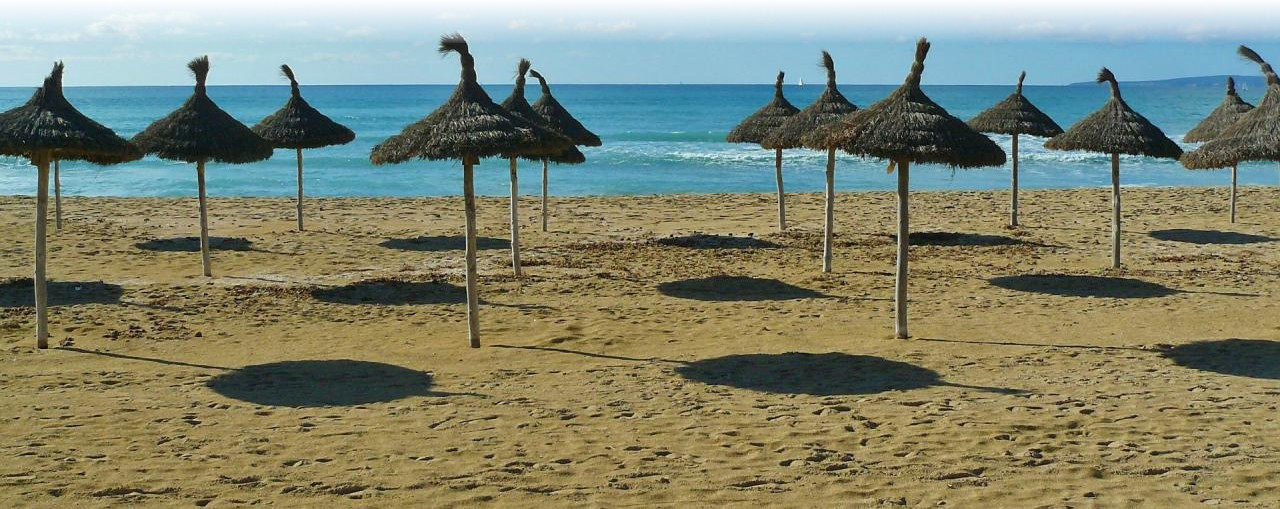
\includegraphics[width=\paperwidth]{sandstrand}\end{minipage}}
\begin{frame}
  \centering

  \Huge \hil{Teil 0}

  \bigskip
  \Large\textbf{Große Zahlen}
  \par
  \bigskip
  \bigskip

  \normalsize

  \hil{300\,000} Augsburger*innen
  \medskip

  \hil{$\boldsymbol{10^{19} = 1\!\underbrace{0\,000\,000\,000\,000\,000\,000}_{\text{$19$ Nullen}}}$}
  Sandkörner auf der Erde
  \medskip

  \hil{$\boldsymbol{10^{80} = 1\!\underbrace{000\ldots000}_{\text{$80$ Nullen}}}$}
  Elementarteilchen im Universum

  % ACTION: video of mass of black hole https://www.youtube.com/watch?v=aIg8gAbqqZc?t=176
  % ACTION: 52!
\end{frame}}

\imgslideHeight{milky-way}
\imgslideHeight{ocean}


\section{Sehr große Zahlen}

\begin{frame}
  \centering

  \Huge \hil{Teil I}

  \bigskip
  \Large\textbf{Sehr große Zahlen}
  \par
  \bigskip

  \normalsize

  \only<1-10>{\[\begin{aligned}
    2 \cdot 4 &= 2 + 2 + 2 + 2 = 8 \\
    2^4 &= 2 \cdot 2 \cdot 2 \cdot 2 = 16 \\
    \pause
    2 \uparrow\uparrow 4 &= 2^{2^{2^2}} = 2^{2^4} = 2^{16} = 65\,536 \\
    \pause
    2 \uparrow\uparrow\uparrow 4 &= 2 \uparrow\uparrow (2 \uparrow\uparrow (2
    \uparrow\uparrow 2)) \pause =
    2 \uparrow\uparrow (2 \uparrow\uparrow 4) \pause =
    2 \uparrow\uparrow 65\,536 \\ \pause &
    \left.\kern-3\nulldelimiterspace
    \begin{array}{@{}l@{}}{}= 2^{2^{\iddots^2}}\end{array} \right\rbrace \text{\scriptsize 65\,536 viele Zweien} \\
    \pause
    2 \uparrow\uparrow\uparrow\uparrow 4 &= 2 \uparrow\uparrow\uparrow (2
    \uparrow\uparrow\uparrow (2 \uparrow\uparrow\uparrow 2)) \pause =
    2 \uparrow\uparrow\uparrow (2 \uparrow\uparrow\uparrow 4) \pause \\
    &= 2 \uparrow\uparrow\uparrow 2^{2^{\iddots^2}} \pause =
    \underbrace{2 \uparrow\uparrow (2 \uparrow\uparrow (2 \uparrow\uparrow (\cdots
    \uparrow\uparrow 2)))}_{\text{$2^{2^{\iddots^2}}$ viele Zweien}}
  \end{aligned}\]}

  \only<11->{\[
    \left.
      \begin{matrix}
        \text{\hil{Grahams Zahl}} &=&3\underbrace{\uparrow \cdots \cdots \cdots \cdots \cdots \uparrow}3 \\
          & &3\underbrace{\uparrow \cdots \cdots \cdots \cdots \uparrow}3 \\[-0.4em]
          & & \underbrace{\qquad \quad \vdots \qquad \quad} \\
          & &3\underbrace{\uparrow \cdots \cdots \uparrow}3 \\
          & &3\uparrow \uparrow \uparrow \uparrow3
      \end{matrix}
    \right \} \text{\small 64 Ebenen}
  \]}

  \only<12->{
    \vspace*{-2.5cm}
    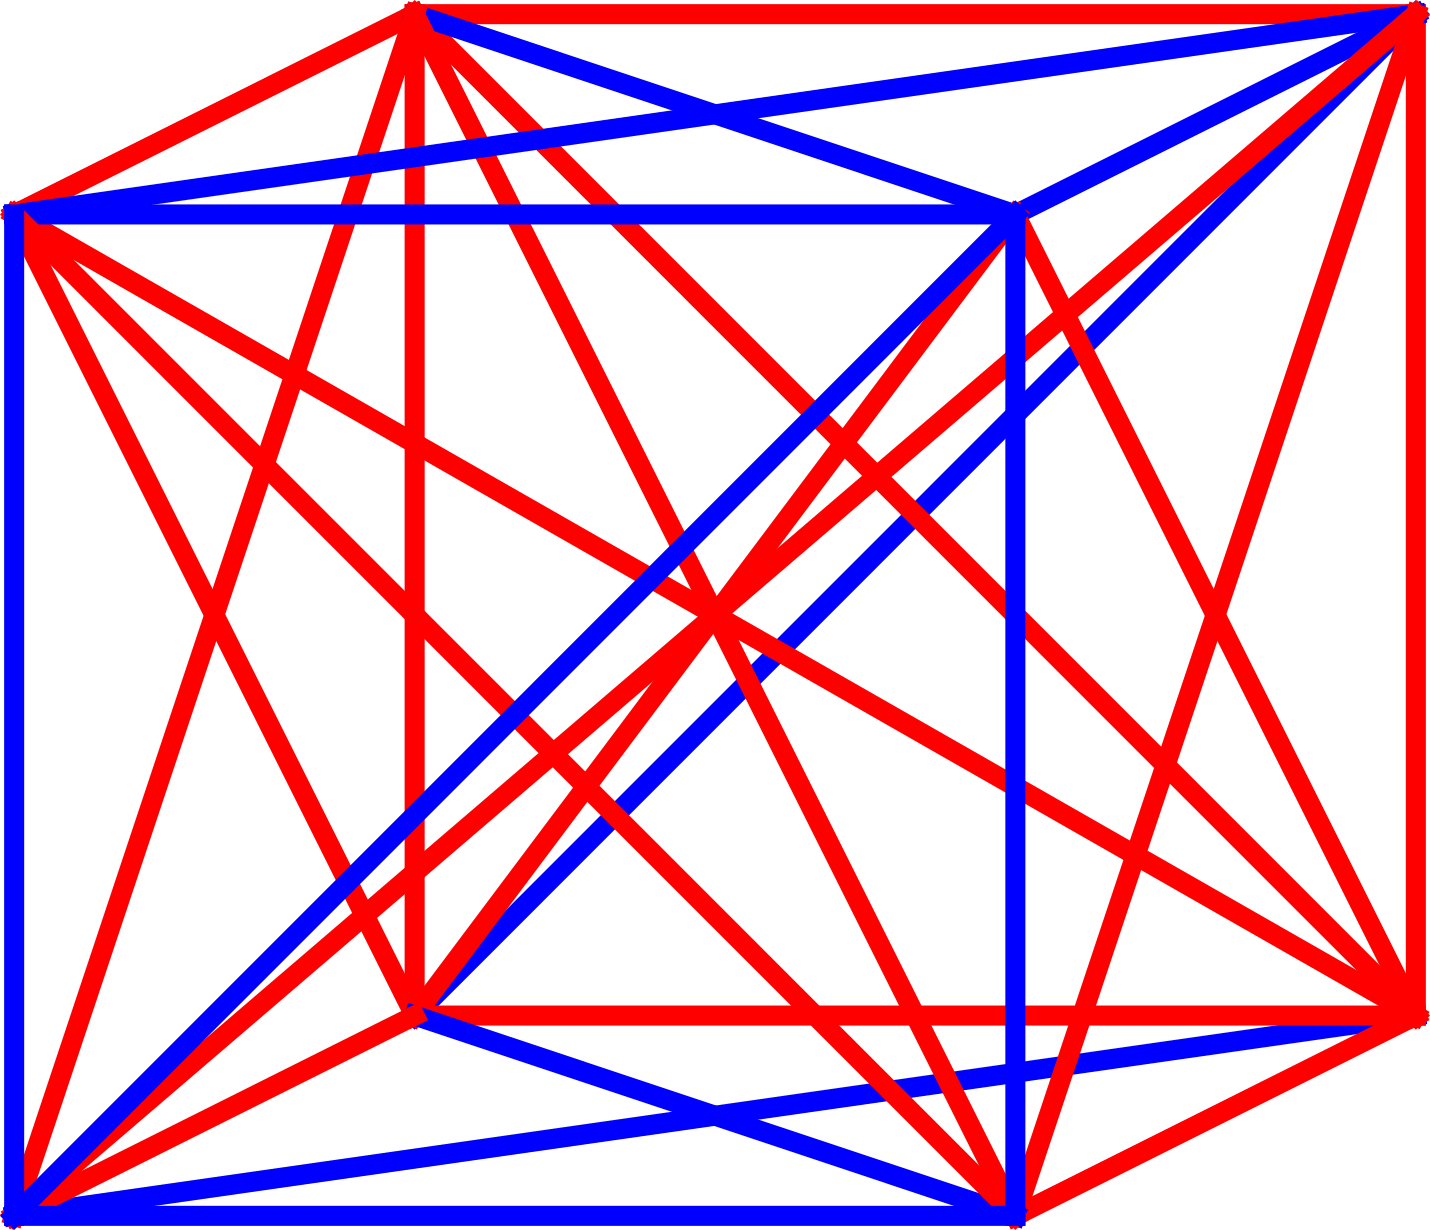
\includegraphics{monophilic-coloring}\hspace*{6cm}
  }
\end{frame}

\begin{frame}[plain]
  \Huge\centering\vfill
  \scalebox{1.5}{$\sqrt{2}^{\sqrt{2}^{\sqrt{2}^{\sqrt{2}^{\iddots}}}} = 2$}
  \pause
  \bigskip
  \bigskip

  \large
  $\sqrt{2 + \sqrt{2 + \sqrt{2 + ...}}} = 2$
  \bigskip

  $\frac{2}{\pi} = \sqrt{\tfrac{1}{2}} \cdot
    \sqrt{\tfrac{1}{2} + \tfrac{1}{2} \sqrt{\tfrac{1}{2}}} \cdot
    \sqrt{\tfrac{1}{2} + \tfrac{1}{2} \sqrt{\tfrac{1}{2} + \tfrac{1}{2}
    \sqrt{\tfrac{1}{2}}}} \cdot \ldots$
  \vfill
\end{frame}


\section{Sehr sehr große Zahlen}

\begin{frame}
  \centering

  \Huge \hil{Teil II}

  \bigskip
  \Large\textbf{Sehr sehr große Zahlen}
  \par
  \bigskip

  \normalsize

  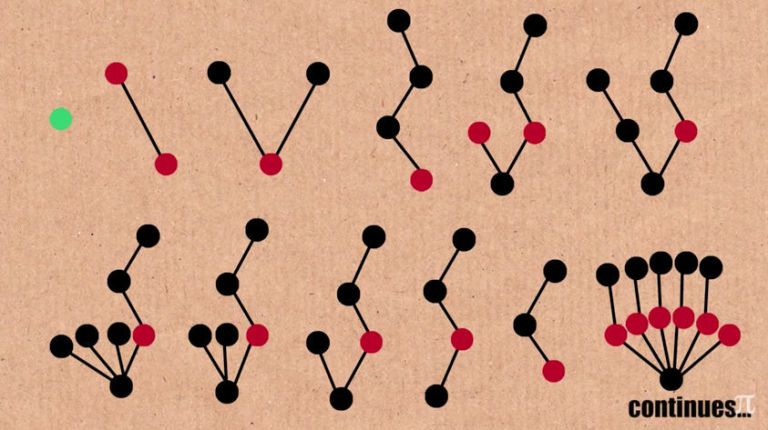
\includegraphics[width=0.8\textwidth]{tree3}
  \bigskip

  Jeder Wald stirbt schlussendlich, bei einer Maximalzahl
  von~\hil{$\boldsymbol{\mathrm{TREE}(3)}$} Bäumen.
\end{frame}


\section{Sehr sehr sehr große Zahlen}

\begin{frame}
  \centering

  \Huge \hil{Teil III}

  \bigskip
  \Large\textbf{Sehr sehr sehr große Zahlen}
  \par
  \bigskip

  \normalsize

  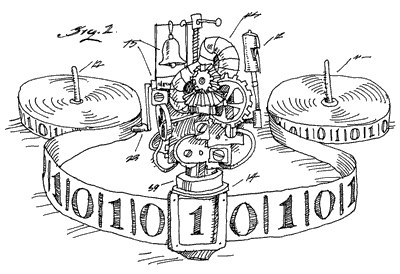
\includegraphics[width=0.3\textwidth]{turing-machine}

  \begin{itemize}\justifying
    \item \hil{$\boldsymbol{\mathrm{BB}(n)}$} ist die größte Zahl, die ein
    terminierendes Computerprogramm bestehend aus~$n$ Bytes berechnen kann.
    \pause
    % ACTION: Values on Wikipedia
    \item Die Busy-Beaver-Funktion ist \hil{unberechenbar}\only<2>{.}
    \visible<3->{und \hil{dominiert} jede berechenbare Funktion.}
    \pause
    \pause
    \item Keine Vermutung über den Wert von~$\mathrm{BB}(1919)$ ist
    mathematisch beweisbar, noch nicht einmal~``$\mathrm{BB}(1919) =
    \heartsuit$'' wobei~$\heartsuit$ der wahre Wert von~$\mathrm{BB}(1919)$ ist.
  \end{itemize}
\end{frame}


%\section{Honorable mentions}
%
%\begin{frame}
%  \centering
%
%  \Huge \hil{Part IV}
%
%  \bigskip
%  \Large\textbf{Honorable mentions}
%  \par
%  \bigskip
%  \normalsize
%
%  \begin{columns}
%    \begin{column}{0.4\textwidth}
%      \card{}{\begin{minipage}{3.3cm}\raggedright The submission of
%      \texttt{\$THAT\textunderscore PERSON}, with the following modification: \ldots\end{minipage}}
%    \end{column}
%
%    \begin{column}{0.4\textwidth}
%      \card{}{\begin{minipage}{4cm}The largest submission of this contest, plus
%      one.\end{minipage}}
%    \end{column}
%
%    \begin{column}{0.4\textwidth}
%      \card{}{\begin{minipage}{4cm}The largest of all \emph{other} submissions
%      of this contest, plus one.\end{minipage}}
%    \end{column}
%  \end{columns}
%\end{frame}


\section{Sehr sehr sehr sehr große Zahlen}

{\usebackgroundtemplate{\begin{minipage}{\paperwidth}\vspace*{0.3cm}\centering\scriptsize\sieve{25}{2}\\\vspace*{3.95cm}\includegraphics[width=\paperwidth]{sun3}\end{minipage}}
\begin{frame}
  \centering

  \Huge \hil{\phantom{Teil IV}}

  \bigskip
  \Large\textbf{Sehr sehr sehr sehr große Zahlen}
  \par
  \bigskip
  \normalsize

  \begin{itemize}\justifying
    \item \hil{$\boldsymbol{\mathrm{Rayo}(n)}$} ist die größte Zahl, die man
    mit höchstens~$n$ Zeichen mathematisch präzise beschreiben kann.
    \item Die Rayo-Funktion \hil{dominiert} \emph{jede}
    mathematisch präzise definierbare Funktion.
  \end{itemize}

  \vfill\hfill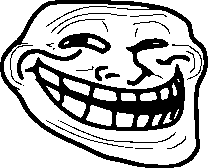
\includegraphics[width=2em]{trollface}
\end{frame}}


\section{Unendlich große Zahlen}

{\usebackgroundtemplate{\begin{minipage}{\paperwidth}\vspace*{0.3cm}\centering\scriptsize\sieve{25}{2}\\\vspace*{3.95cm}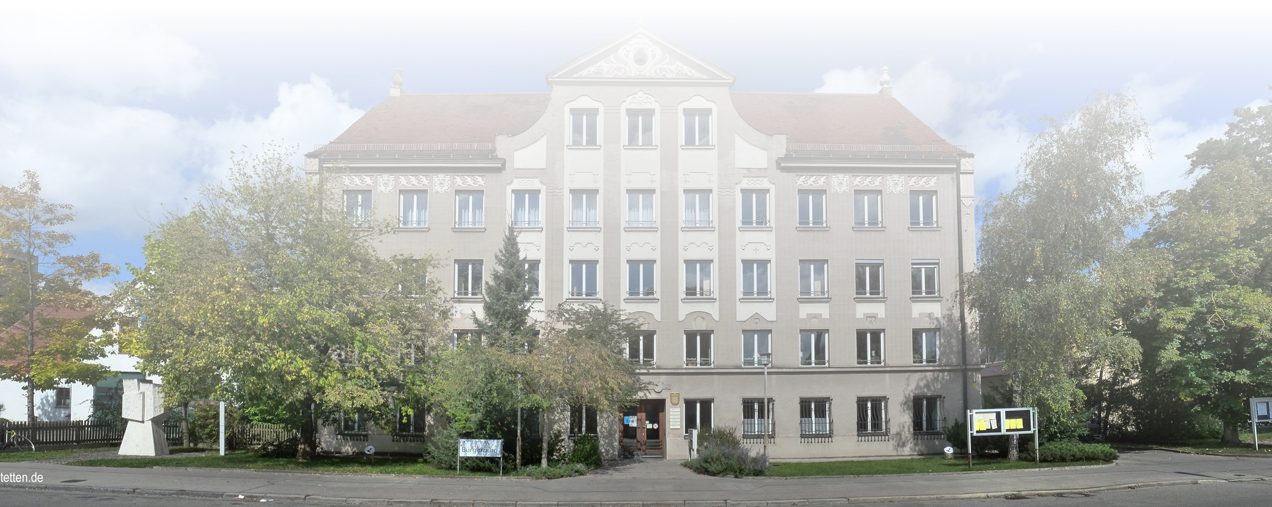
\includegraphics[width=\paperwidth]{buergerbuero-haunstetten}\end{minipage}}
\begin{frame}
  \centering

  \Huge \hil{\phantom{Teil V}}

  \bigskip
  \Large\textbf{Unendlich große Zahlen}
  \par
  \bigskip

  \large\hil{Ordinalzahlen}
  \par

  messen Anordnung
\end{frame}}

{\usebackgroundtemplate{\parbox[c][\paperheight][c]{\paperwidth}{\vspace*{0.2cm}\hspace*{-0.2cm}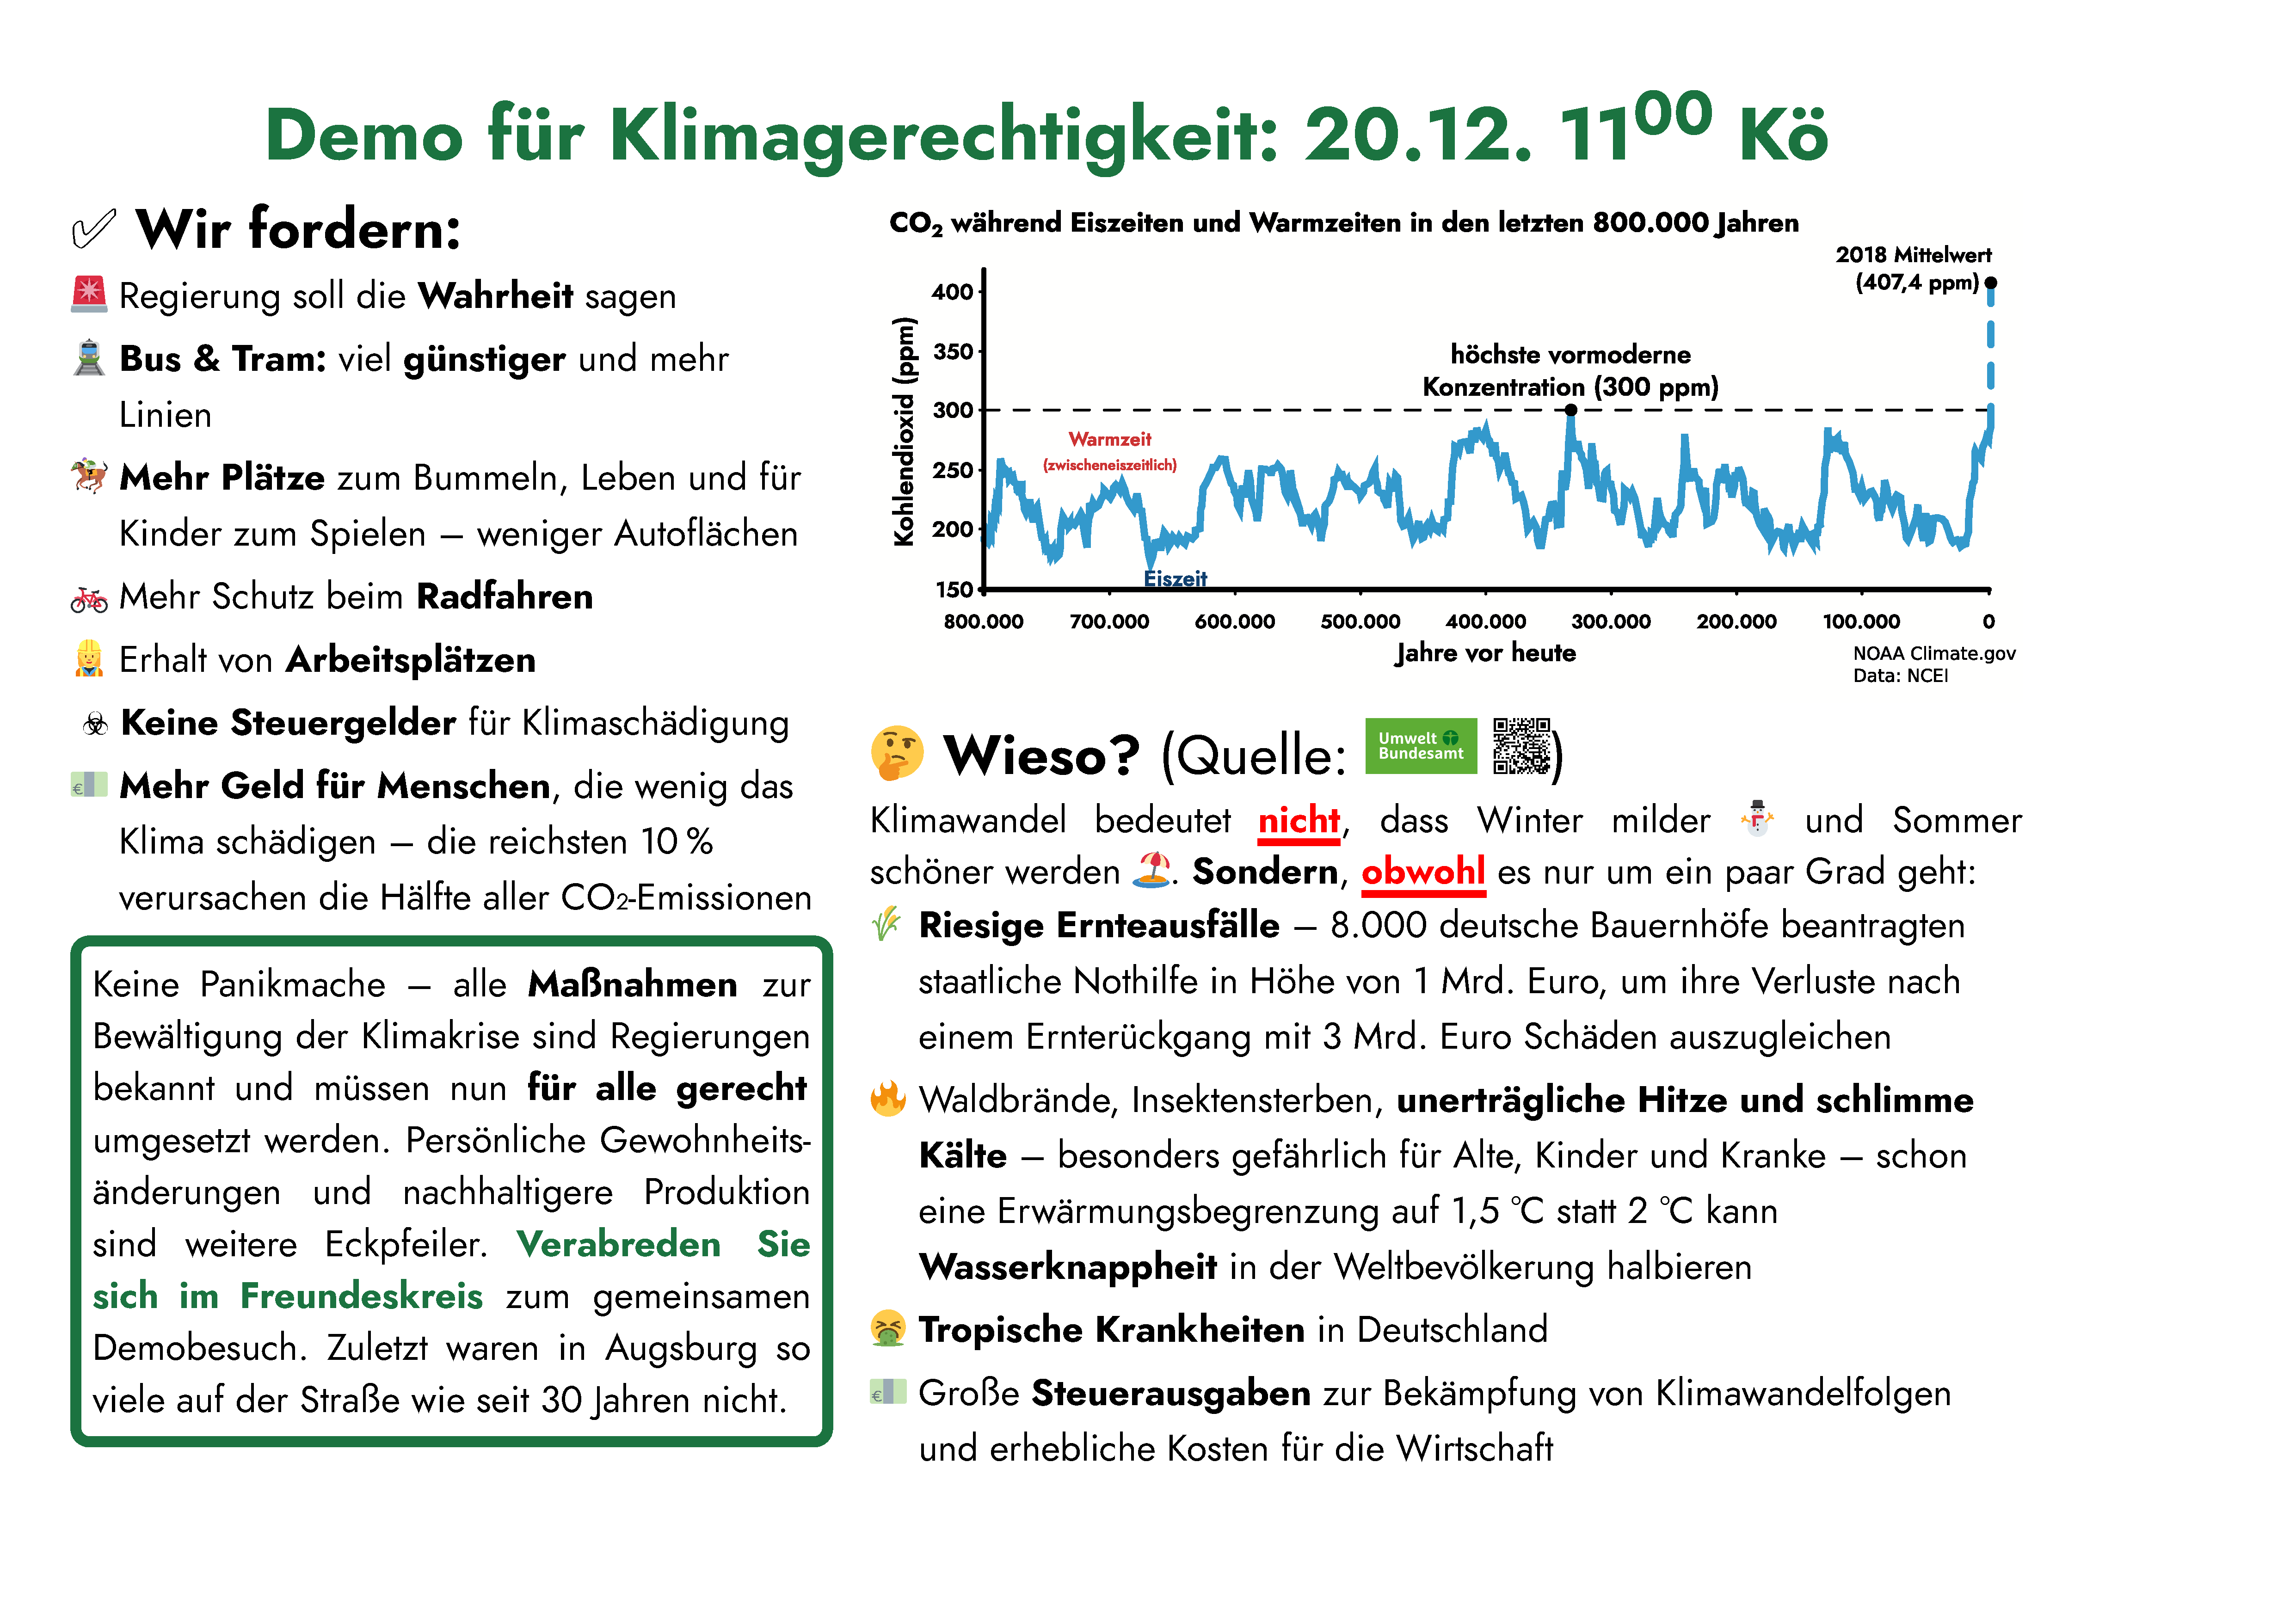
\includegraphics[height=1.07\paperheight]{fff-2019-12-20}}}\begin{frame}[plain]\end{frame}}
\end{document}


BEACHTEN:
* Black hole
* Wikipedia-Werte BB
* Nutzen
* Ziffern Graham

NÄCHSTES MAL BESSER MACHEN:
* Beim BB- und Rayo-Kapitel mehr Drive haben.
* Krassheit von Rayo besser zur Geltung bringen.
* Nutzen vorbringen!
* Ruhiger formale Systeme erklären?
* "Calbrating the finite by using the infinite" (fast-growing hierarchy)
